\section{Experimental results}
\label{sec:experimental_results}

\subsection{Dataset}
\label{sec:dataset}

Experiments from this paper use the Microsoft MSRC V2 dataset \cite{microsoft_msrc}. The dataset consists of 591
images classified into 20 different categories. However, there are some images that have incorrect or confusing
categories. Because of this the precision values for a given feature extractor might be higher that its actual value.

\subsection{Results}
\label{sec:results}

\subsubsection{Global Color Histogram}
\label{sec:results_gch}

One of the feature extraction methods used in the experiments was the Global Color Histogram. Changing the color
histogram quantization can be observed in Figure \ref{fig:gch_varyingmap} and Color Quantization 5 is noted to have
the highest mean average precision. The best average PR curve for the Global Color Histogram descriptor was for
quantization 5 as seen in Figure \ref{fig:gch_mean_pr_graph_q5}.

\begin{figure}[htbp]
  \begin{center}
    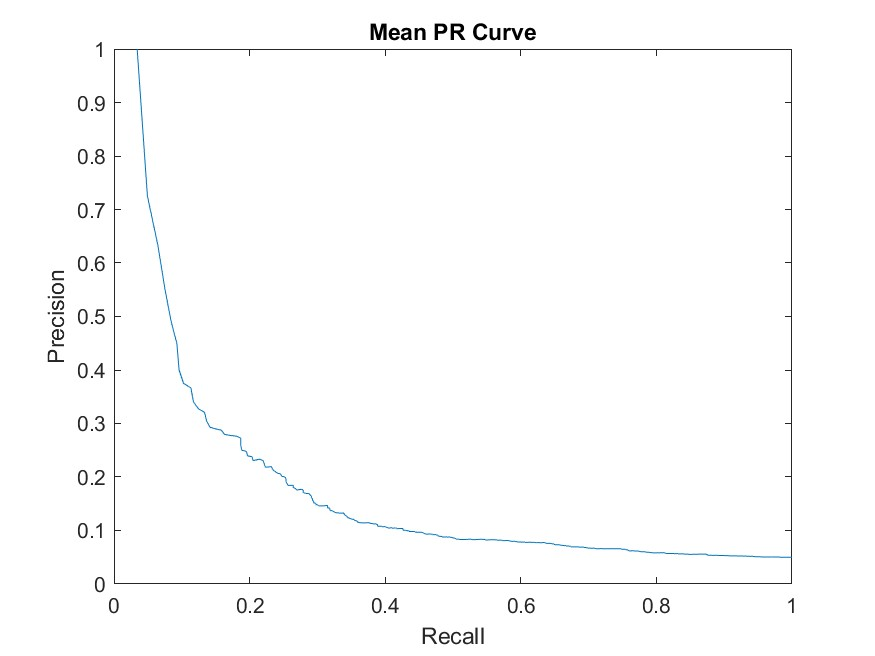
\includegraphics[width=0.5\textwidth]{./assets/plots/Global_Color_Histogram/mean_pr_graph_q4.jpg}
    \caption{Mean Precision-Recall curve with $Q$=5}
    \label{fig:gch_mean_pr_graph_q5}
  \end{center}
\end{figure}

\begin{figure}[htbp]
  \begin{center}
    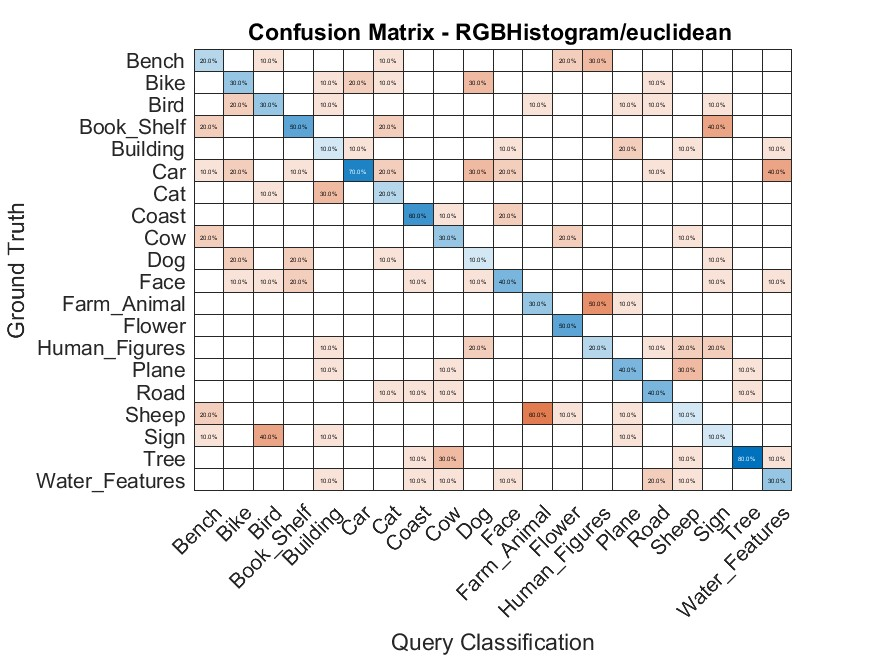
\includegraphics[width=0.5\textwidth]{./assets/plots/Global_Color_Histogram/confusion_matrix_n10.jpg}
    \caption{Confusion matrix for Global Color Histogram with $Q$=5}
    \label{fig:gch_confmat}
  \end{center}
\end{figure}

\begin{figure}[htbp]
  \begin{center}
    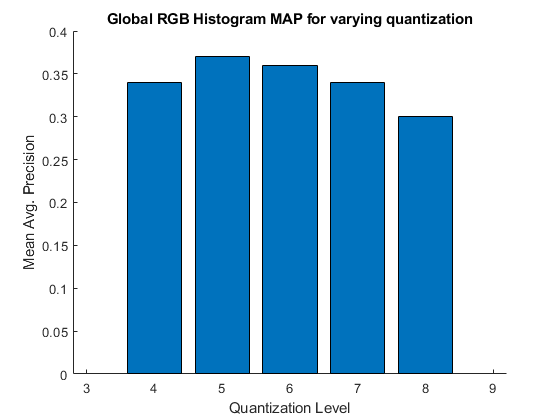
\includegraphics[width=0.5\textwidth]{./assets/plots/Global_Color_Histogram/map_varying_q.png}
    \caption{MAP values for varying Color Quantization}
    \label{fig:gch_varyingmap}
  \end{center}
\end{figure}


\subsubsection{Spacial Grid with Color and Texture Histogram}
\label{sec:results_spacial_grid}

Spacial Grid with Color and Texture Histogram was used to explore best grid sizes and color/texture quantizations for
the Spacial Grid technique. As shown in Figure \ref{fig:sgch_varyingmap}, a 3x3 grid has the best mean average
precision.

\begin{figure}[htbp]
  \begin{center}
    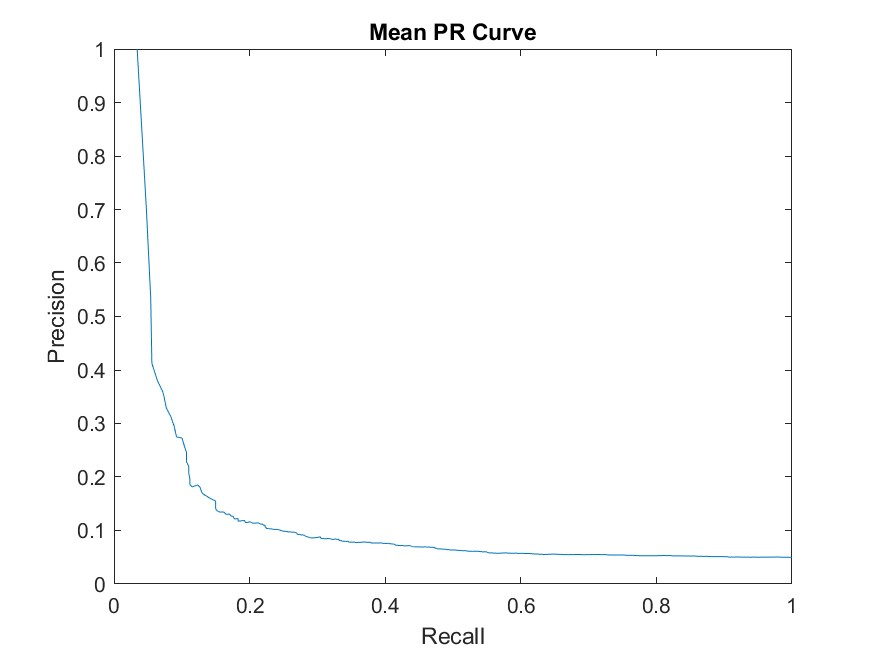
\includegraphics[width=0.5\textwidth]{./assets/plots/Spacial_Grid_Color_Histogram/mean_pr_graph_3x3_4q.jpg}
    \caption{Mean Precision-Recall curve; 3x3 grid; $Q$=4}
    \label{fig:sgch_mean_pr_graph_q4}
  \end{center}
\end{figure}

\begin{figure}[htbp]
  \begin{center}
    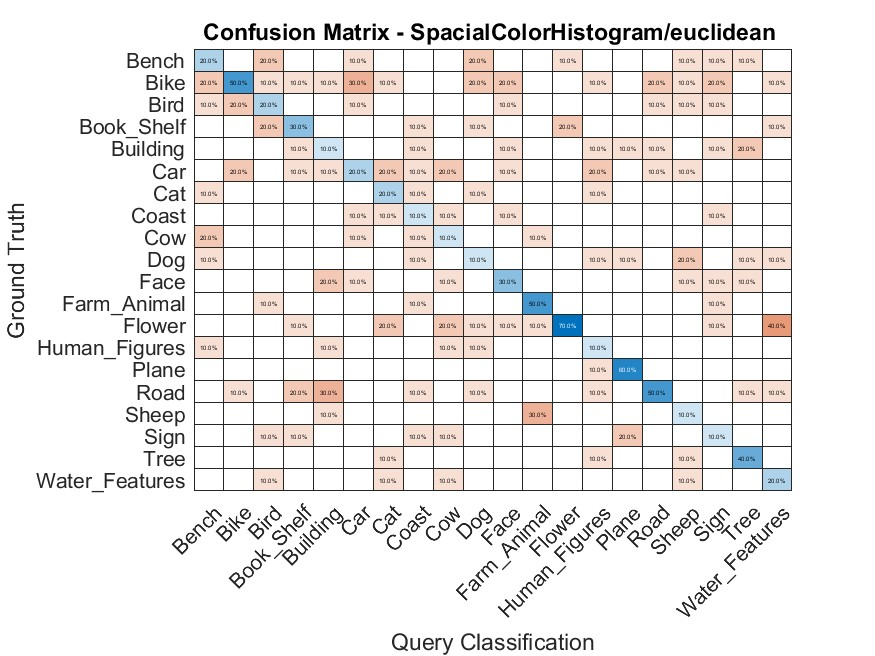
\includegraphics[width=0.5\textwidth]{./assets/plots/Spacial_Grid_Color_Histogram/confusion_matrix.jpg}
    \caption{Confusion matrix for Spacial Grid with Color Histogram; 3x3 grid; $Q$=4}
    \label{fig:sgch_confmat}
  \end{center}
\end{figure}

\begin{figure}[htbp]
  \begin{center}
    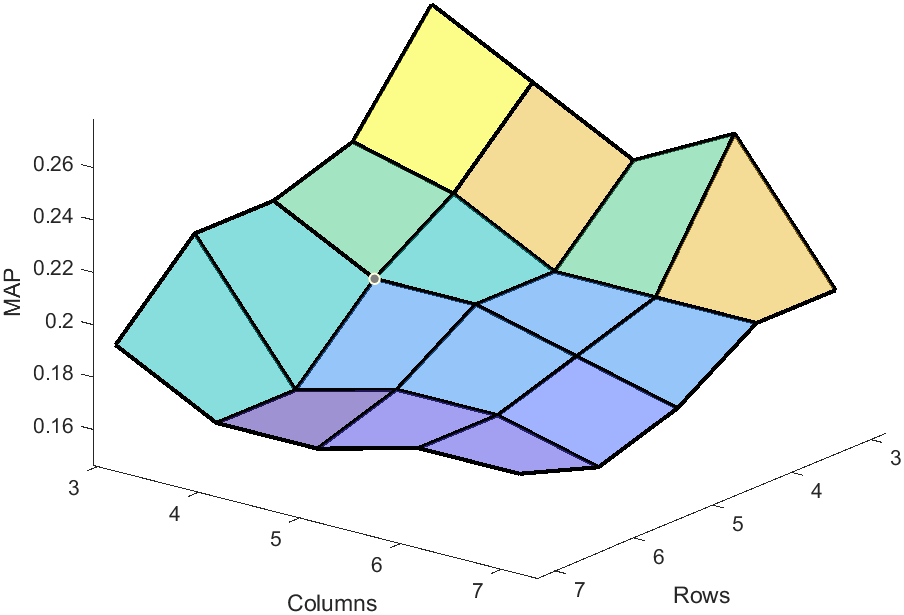
\includegraphics[width=0.5\textwidth]{./assets/plots/Spacial_Grid_Color_Histogram/map_varying_grid.png}
    \caption{MAP values for varying grid rows and columns}
    \label{fig:sgch_varyingmap}
  \end{center}
\end{figure}

\subsubsection{Convolutional Neural Network}
\label{sec:results_cnn}

Convolutional Neural Networks extracted desirable features. This experiment used AlexNet's fc7 layer to extract feature
information. Figure \ref{fig:cnn_output} shows an impressive result using CNNs.

\begin{figure}[htbp]
  \begin{center}
    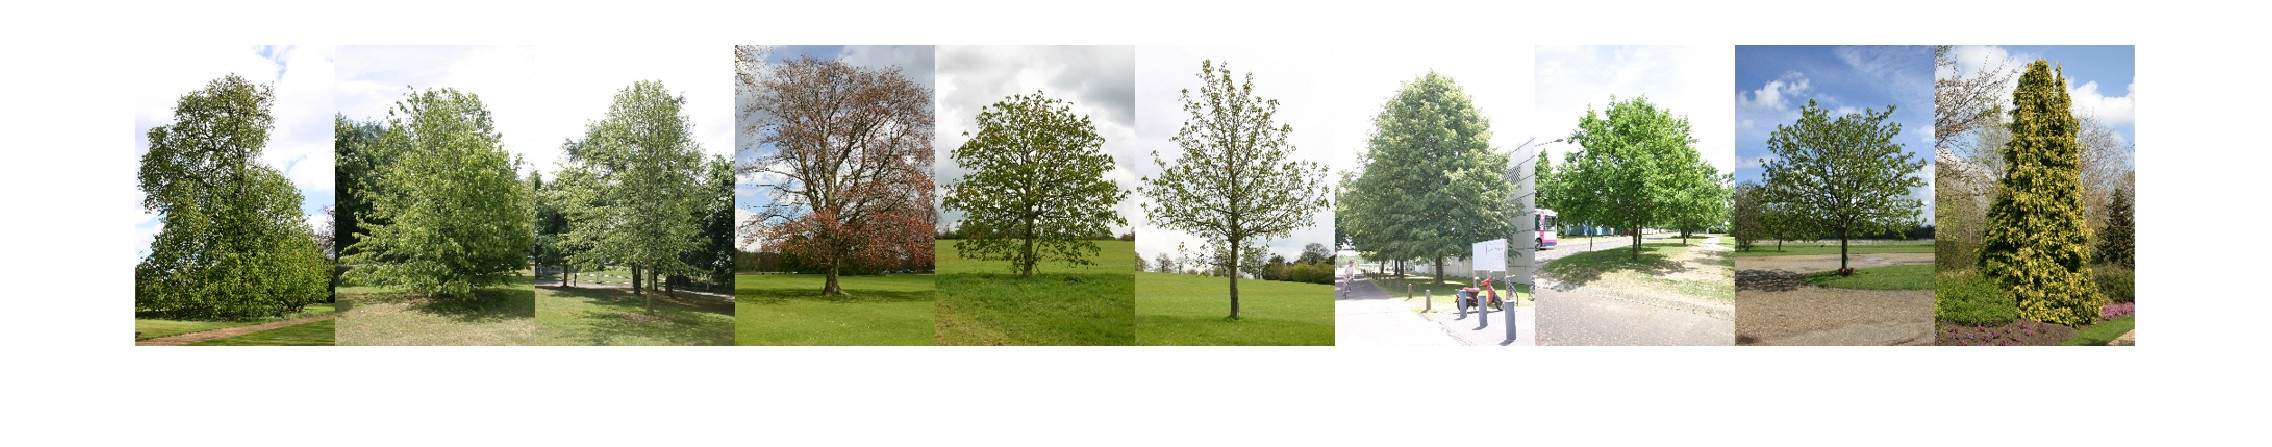
\includegraphics[width=0.9\textwidth]{./assets/plots/CNN/search_output.jpg}
    \caption{Search output using a CNN descriptor; AlexNet}
    \label{fig:cnn_output}
  \end{center}
\end{figure}

\begin{figure}[htbp]
  \begin{center}
    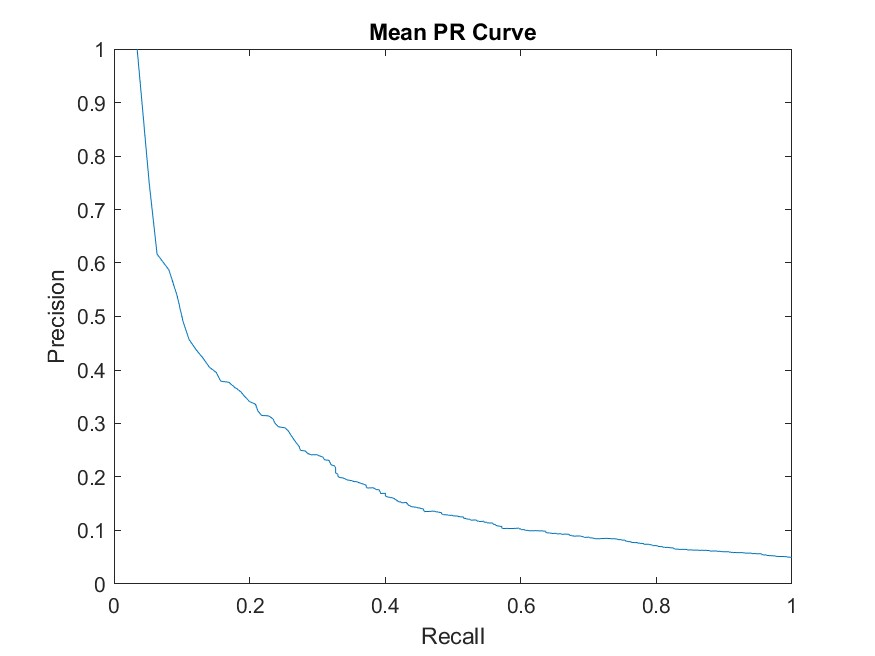
\includegraphics[width=0.5\textwidth]{./assets/plots/CNN/mean_pr_graph.jpg}
    \caption{Mean Precision-Recall curve; AlexNet}
    \label{fig:cnn_mean_pr_graph_q4}
  \end{center}
\end{figure}

\begin{figure}[htbp]
  \begin{center}
    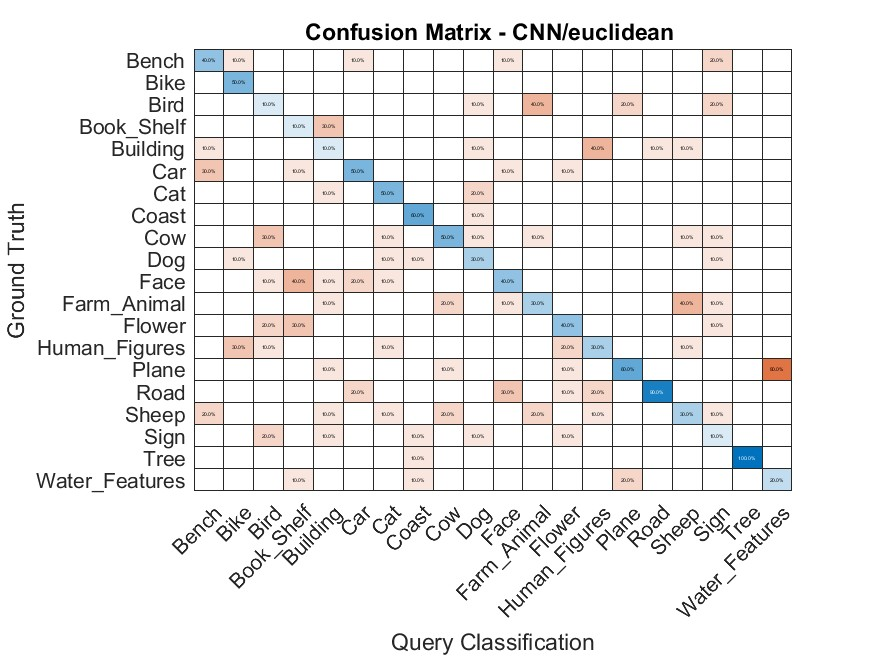
\includegraphics[width=0.5\textwidth]{./assets/plots/CNN/confusion_matrix.jpg}
    \caption{Confusion matrix for CNN feature extractor; AlexNet}
    \label{fig:cnn_confmat}
  \end{center}
\end{figure}
